\documentclass[12pt,b5paper]{ltjsarticle}

%\usepackage[margin=15truemm, top=5truemm, bottom=5truemm]{geometry}
%\usepackage[margin=10truemm,left=15truemm]{geometry}
\usepackage[margin=10truemm]{geometry}

\usepackage{amsmath,amssymb}
%\pagestyle{headings}
\pagestyle{empty}

%\usepackage{listings,url}
%\renewcommand{\theenumi}{(\arabic{enumi})}

\usepackage{graphicx}

\usepackage{tikz}
%\usetikzlibrary {arrows.meta}
%\usepackage{wrapfig}
%\usepackage{bm}

% ルビを振る
\usepackage{luatexja-ruby}	% required for `\ruby'

%% 核Ker 像Im Hom を定義
%\newcommand{\Img}{\mathop{\mathrm{Im}}\nolimits}
%\newcommand{\Ker}{\mathop{\mathrm{Ker}}\nolimits}
%\newcommand{\Hom}{\mathop{\mathrm{Hom}}\nolimits}

%\DeclareMathOperator{\Rot}{rot}
%\DeclareMathOperator{\Div}{div}
%\DeclareMathOperator{\Grad}{grad}
%\DeclareMathOperator{\arcsinh}{arcsinh}
%\DeclareMathOperator{\arccosh}{arccosh}
%\DeclareMathOperator{\arctanh}{arctanh}

\usepackage{url}

%\usepackage{listings}
%
%\lstset{
%%プログラム言語(複数の言語に対応,C,C++も可)
%  language = Python,
%%  language = Lisp,
%%  language = C,
%  %背景色と透過度
%  %backgroundcolor={\color[gray]{.90}},
%  %枠外に行った時の自動改行
%  breaklines = true,
%  %自動改行後のインデント量(デフォルトでは20[pt])
%  breakindent = 10pt,
%  %標準の書体
%%  basicstyle = \ttfamily\scriptsize,
%  basicstyle = \ttfamily,
%  %コメントの書体
%%  commentstyle = {\itshape \color[cmyk]{1,0.4,1,0}},
%  %関数名等の色の設定
%  classoffset = 0,
%  %キーワード(int, ifなど)の書体
%%  keywordstyle = {\bfseries \color[cmyk]{0,1,0,0}},
%  %表示する文字の書体
%  %stringstyle = {\ttfamily \color[rgb]{0,0,1}},
%  %枠 "t"は上に線を記載, "T"は上に二重線を記載
%  %他オプション:leftline,topline,bottomline,lines,single,shadowbox
%  frame = TBrl,
%  %frameまでの間隔(行番号とプログラムの間)
%  framesep = 5pt,
%  %行番号の位置
%  numbers = left,
%  %行番号の間隔
%  stepnumber = 1,
%  %行番号の書体
%%  numberstyle = \tiny,
%  %タブの大きさ
%  tabsize = 4,
%  %キャプションの場所("tb"ならば上下両方に記載)
%  captionpos = t
%}

%\usepackage{cancel}
%\usepackage{bussproofs}
%\usepackage{proof}

\begin{document}

\hrulefill

\begin{description}
 \item[25]
            次の4種類の機械が有り、
            aからdへ4回処理を行うことで製品が作られるとする。
            \begin{tabular}{|c||c|c|c|c|}
             \hline
             種類 & 機械a & 機械b & 機械c & 機械d \\
             \hline
             能力 & 200個/分 & 300個/分 & 150個/分 & 240個/分 \\
             \hline
            \end{tabular}

            機械a~dを計17台用いて、
            30,000個の製品を作る時、
            必要な時間は最短で約何分であるか?

            \dotfill

            各機械間の製造能力の差が
            出来るだけ小さい方が製造効率が良い。
            その為、
            生産能力を同じにする様に機械を配置すると次のようになる。

            \begin{tabular}{|c|c|c|c|c|}
             \hline
             種類 & 機械a & 機械b & 機械c & 機械d \\
             \hline
             台数 & 6台 & 4台 & 8台 & 5台 \\
             \hline
             総生産能力 & 1200個/分 & 1200個/分 & 1200個/分 & 1200個/分 \\
             \hline
            \end{tabular}

            この場合、計23台必要である。

            計17台にする為、
            6台減らす。

            \begin{tabular}{|c|c|c|c|c|}
             \hline
             種類 & 機械a & 機械b & 機械c & 機械d \\
             \hline
             台数 & 4台 & 3台 & 6台 & 4台 \\
             \hline
             総生産能力 & 800個/分 & 900個/分 & 900個/分 & 960個/分 \\
             \hline
            \end{tabular}

            生産は能力の最も低い部分に影響を受けるので、
            30,000個の生産時間は次の式で求められる。
            \begin{equation}
             30000 \div 800 = 37.5
            \end{equation}

            よって、30,000個の生産は37.5分かかる。

            \hrulefill

 \item[28]

            1辺が6の立方体$ABCD-EFGH$を考える。

            辺$EH$上に$EI=4$となるように点$I$を取り、
            辺$FG$上に$FJ=2$となるように点$J$を取る。

            この時、立体$ACIJ$の体積を求めよ。

            \dotfill

            立方体から立体$ACIJ$を除くと2つの立体
            (頂点$B$を含む立体と頂点$D$を含む立体)に分かれる。

            \textbf{$B$を含む立体}

            $A$を頂点とする2つの四角錐
            ($A-EFJI$と$A-BFJC$)
            に分かれるので、
            それぞれの体積を求める。

            \begin{description}
             \item[$A-EFJI$]
                        底面$EFJI$は
                        $2\times 6 + (4-2)\times 6 \div 2 = 18$である。
                        高さは$AE=6$であるので、
                        $18\times 6 \div 3 = 36$
             \item[$A-BFJC$]
                        底面$BFJC$は
                        $2\times 6 + (6-2)\times 6 \div 2 = 24$である。
                        高さは$AB=6$であるので、
                        $24\times 6 \div 3 = 48$
            \end{description}

            \textbf{$D$を含む立体}

            $C$を頂点とする2つの四角錐
            ($C-DHIA$と$C-GHIJ$)
            に分かれるので、
            それぞれの体積を求める。

            \begin{description}
             \item[$C-DHIA$]
                        底面$DHIA$は
                        $2\times 6 + (6-2)\times 6 \div 2 = 24$である。
                        高さは$CD=6$であるので、
                        $24\times 6 \div 3 = 48$
             \item[$C-GHIJ$]
                        底面$GHIJ$は
                        $2\times 6 + (4-2)\times 6 \div 2 = 18$である。
                        高さは$CG=6$であるので、
                        $18\times 6 \div 3 = 36$
            \end{description}

            立方体の体積は$6^3=216$であるので、
            求めるべき体積は4つの四角錐を除くことで得られる。

            \begin{equation}
             216-(36+48+48+36) = 48
            \end{equation}

            \hrulefill

 \item[30]

            4つの正方形を横に並べる。

            次のように2つの三角形を作った時、
            角度$x$を求めよ。
            \begin{center}
             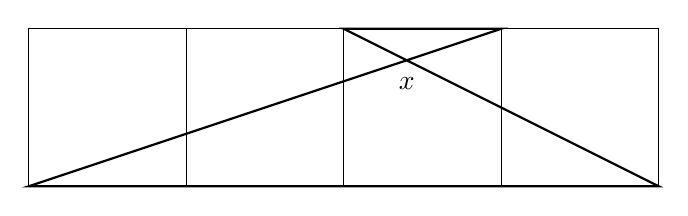
\begin{tikzpicture}
              \draw (0,0) rectangle (2,2);
              \draw (2,0) rectangle (4,2);
              \draw (4,0) rectangle (6,2);
              \draw (6,0) rectangle (8,2);

              \draw[thick] (0,0) -- (6,2) -- (4,2) -- (8,0) -- cycle;
              \node(P) at (4.8, 1.3) {$x$};
             \end{tikzpicture}
            \end{center}

            \dotfill

            3つ目の正方形に描かれている三角形を分けて横にずらすと
            次のようになる。
            \begin{center}
             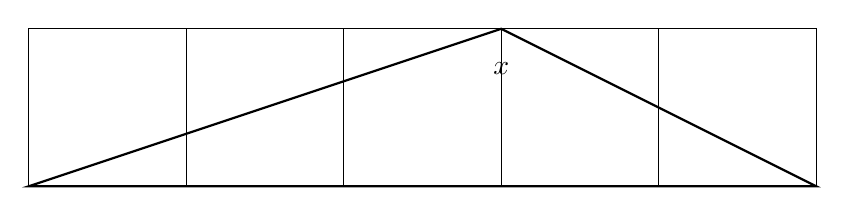
\begin{tikzpicture}
              \draw (0,0) rectangle (2,2);
              \draw (2,0) rectangle (4,2);
              \draw (4,0) rectangle (6,2);
              \draw (6,0) rectangle (8,2);
              \draw (8,0) rectangle (10,2);

              \draw[thick] (0,0) -- (6,2) -- (10,0) -- cycle;
              \node(P) at (6, 1.5) {$x$};
             \end{tikzpicture}
            \end{center}

            角度は変わらないので、この図の角度$x$を求める。

            $x$を挟んでいる辺の長さは三平方の定理より
            それぞれ$\sqrt{10},\;\sqrt{5}$である。

            余弦定理より、$\cos{x}$を求める。
            \begin{equation}
             \cos{x}=\frac{\sqrt{10}^{2}+\sqrt{5}^{2} - 5^2}{2\times \sqrt{10}\times\sqrt{5}}
              =-\frac{1}{\sqrt{2}}
            \end{equation}

            これにより$x$は$135^{\circ}$である。


\end{description}

\hrulefill

\end{document}

